\documentclass[aspectratio=169,9pt]{beamer}
\usepackage[UTF8]{ctex}
\usepackage{minted}
\title{强化学习单标的择时策略}
\date[ISPN ’80]{2022/8/25}
\author[LiuShihao]{刘世豪}

\usetheme{atomus}

\begin{document}

\begin{frame}[plain]            % plain disables headline and footline
\titlepage
\end{frame}

\AtEndDocument
{
  \begin{frame}[plain]          % plain disables headline and footline
    \usebeamertemplate{endpage}
  \end{frame}
}

\begin{frame}
  \frametitle{引入随机性}
  使Agent面对的环境更复杂,增加泛化能力
  \begin{enumerate}
  \item 每个episode的起始位置随机    --- (有一定作用)
  \item 环境每一步随机向前走(跳)n个交易日 --- (无效)
  \end{enumerate}
\end{frame}

\begin{frame}
  \frametitle{测试其它指标}
  \begin{columns}
    \begin{column}{0.5\textwidth}
      \begin{enumerate}
      \item 成分股涨跌比率
      \item 上涨集中度(成分股涨幅超过benchmark的比例)
      \end{enumerate}
    \end{column}
    \begin{column}{0.5\textwidth}
      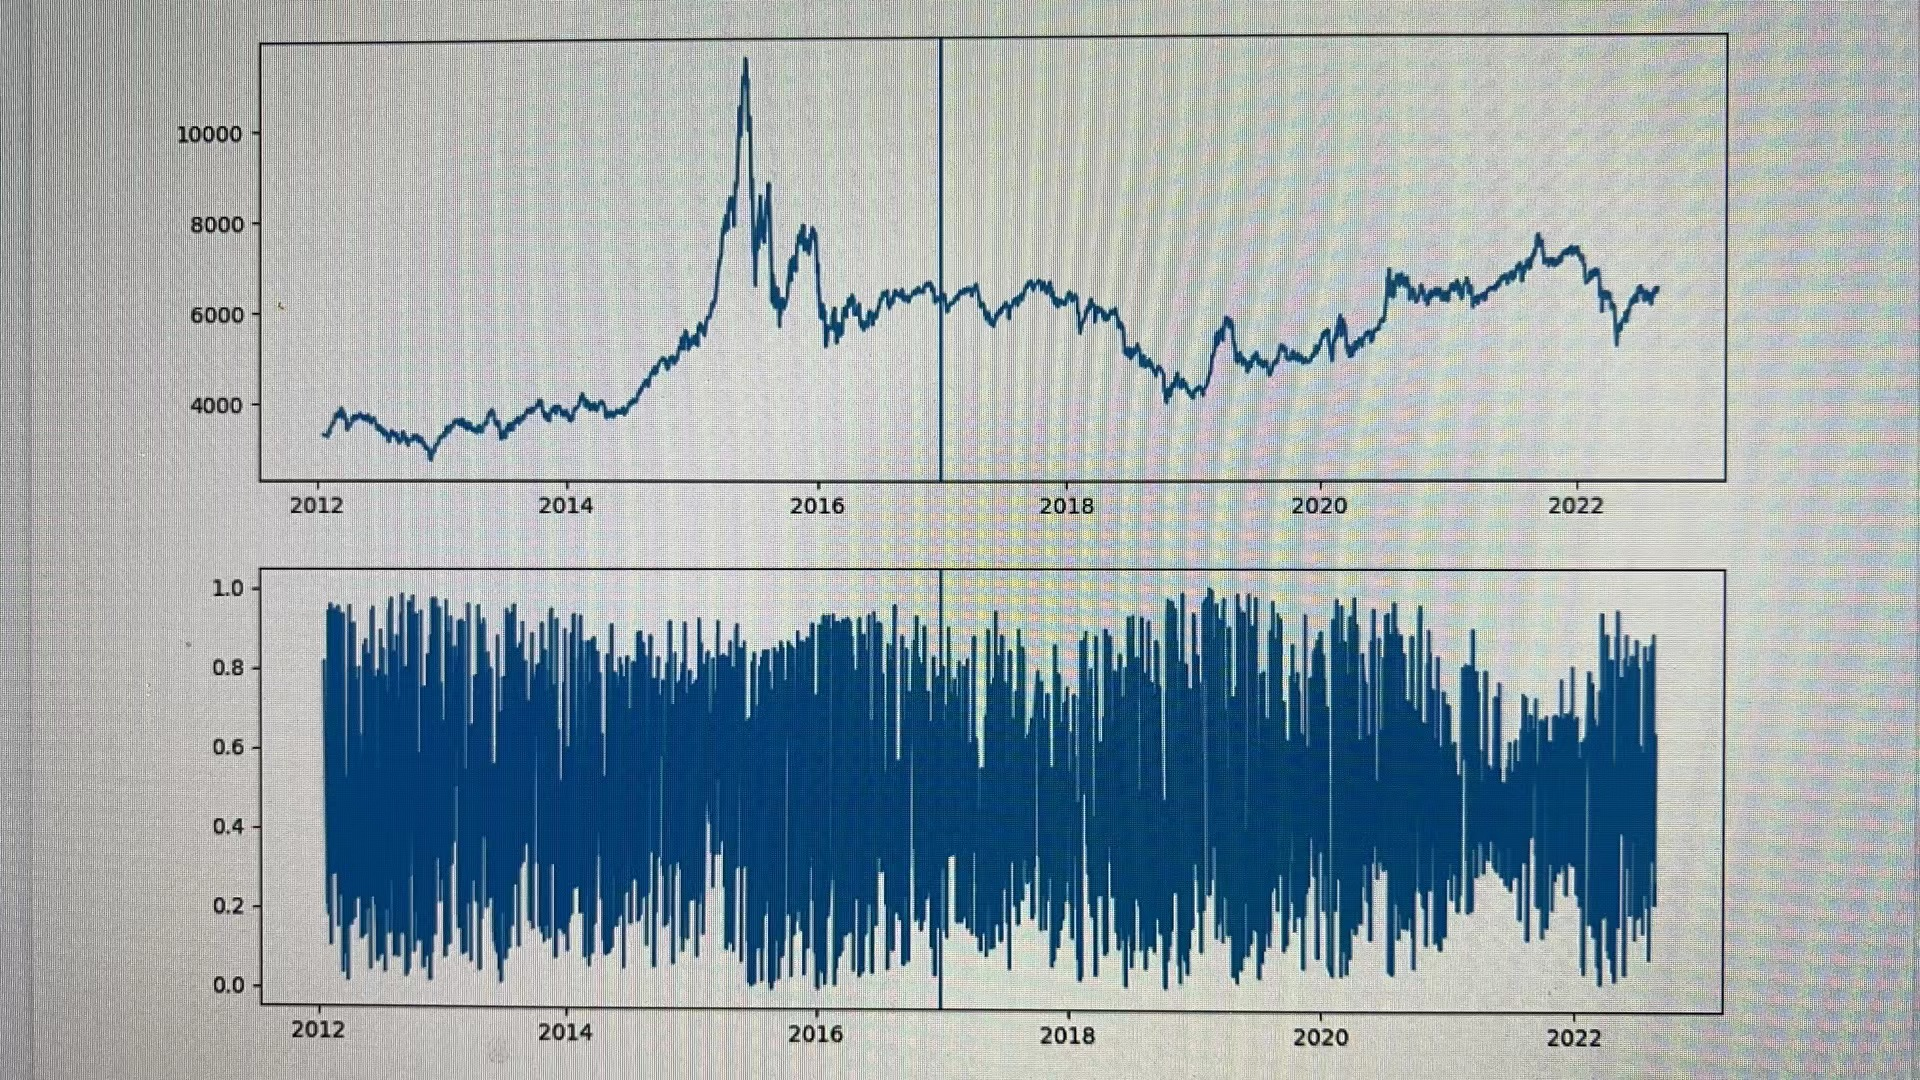
\includegraphics[height=0.4\paperheight]{media/rise-rates.jpg}
      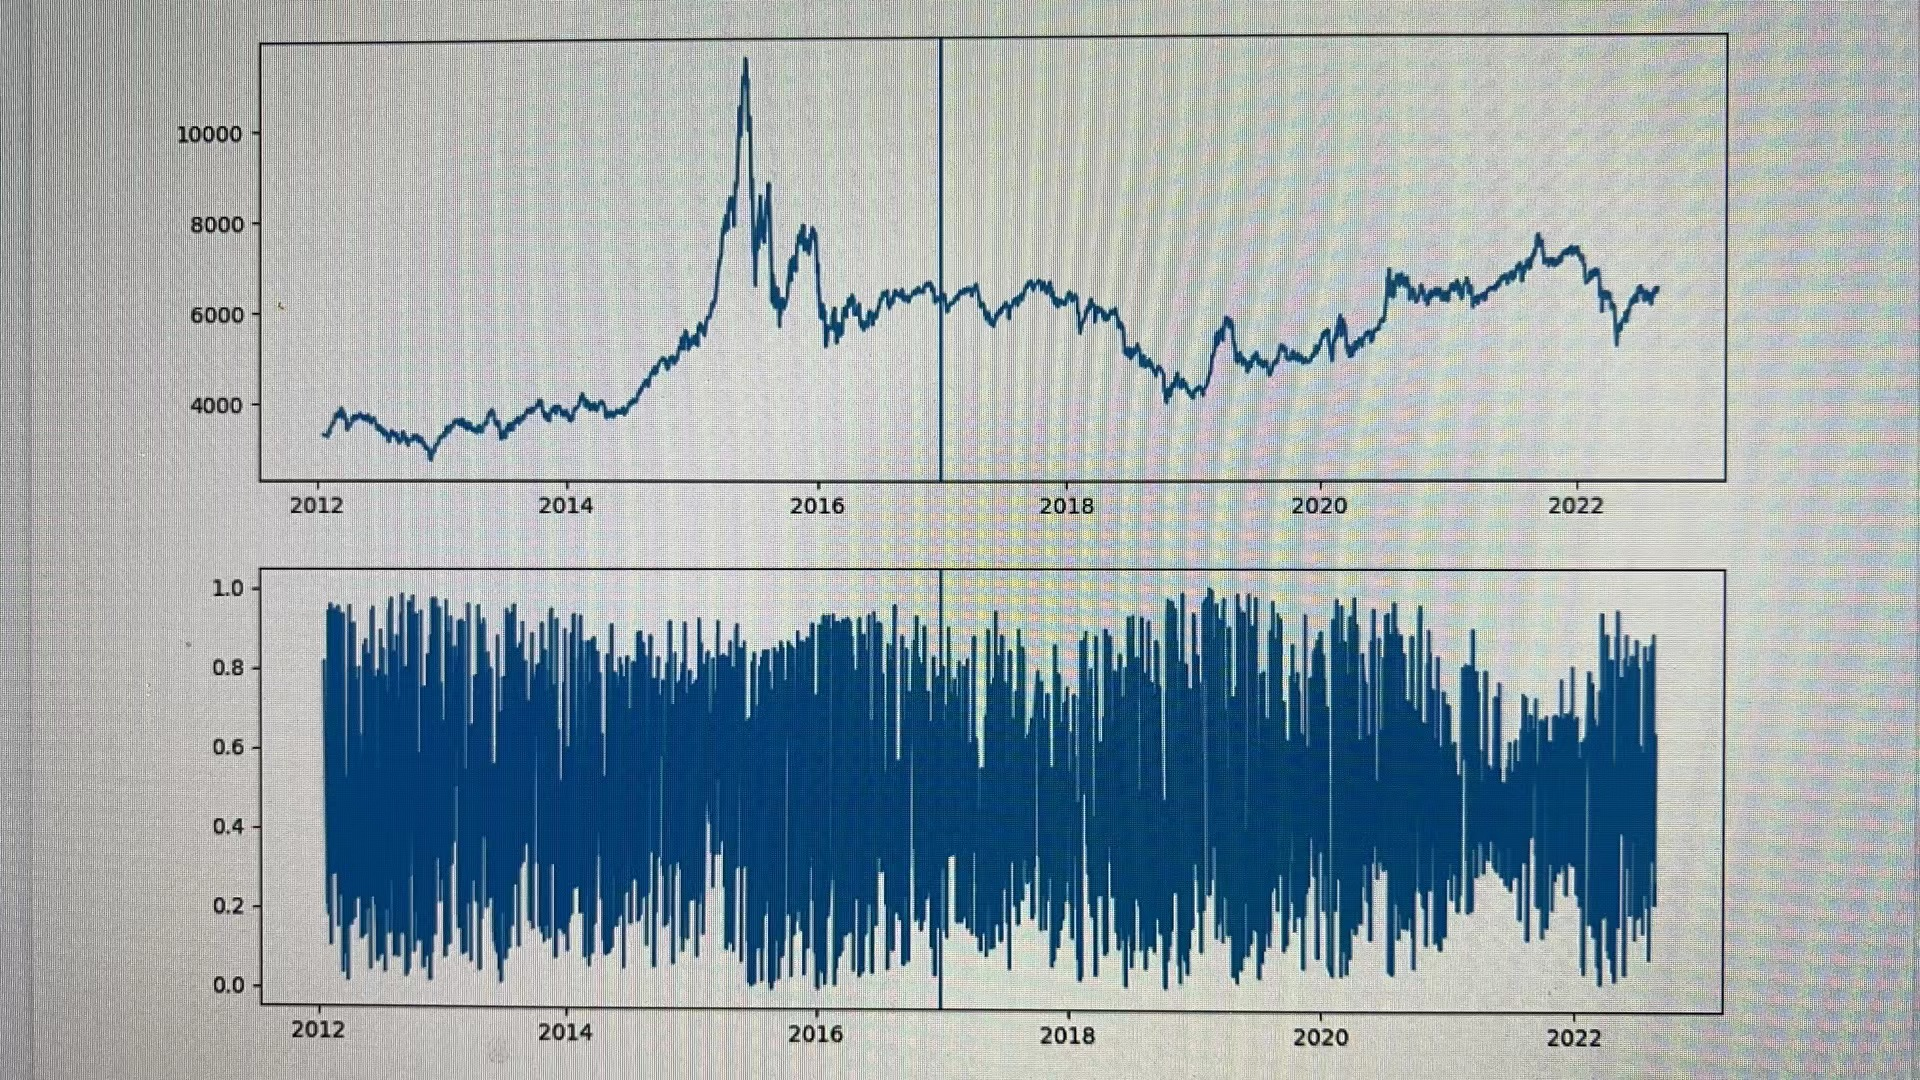
\includegraphics[height=0.4\paperheight]{media/rise-rates.jpg}
    \end{column}
  \end{columns}
\end{frame}

\begin{frame}[fragile]
  \begin{columns}
    \begin{column}{0.4\textwidth}
      In C++:
      \begin{minted}[fontsize=\footnotesize]{cpp}
int main() {
  std::out << "Hello world!" << std::endl;
  return 0;
}
      \end{minted}
    \end{column}
    \begin{column}{0.4\textwidth}
      In Python:
      \begin{minted}[fontsize=\footnotesize]{python}
if __name__ == '__main__':
    print('Hello world!')
      \end{minted}
    \end{column}
  \end{columns}
\end{frame}

\end{document}
%%% Local Variables:
%%% mode: latex
%%% TeX-master: t
%%% End:
